\newpage % Эта команда начинает новую страницу
\chapter{Тема лекции}% Эта команда начинает первую лекцию. В фигурных скобках нужно
% записать тему лекции. Эта тема лекции автоматически получит порядковый номер и
% автоматически добавится в раздел <<Содержание>>. Лекций можно создавать сколько угодно.
% Для создания новой лекции скопируйте и вставьте (или наберите с клавиатуры) команду
% \chapter{Тема лекции} в любую часть рабочего файла. Можете смело менять местами лекции --
% вся нумерация после очередной компиляции поменяется автоматически.

% При необходимости здесь можно разместить любой текст

\section{Название параграфа}% Эта команда начнет раздел, который будем далее условно называть
% параграф. В роли параграфа будет выступать структурная часть лекции (отдельный раздел,
% вопрос и т.п.). В фигурных скобках нужно вписать название параграфа. Параграф автоматически
% получит порядковый номер, который будет состоять из двух чисел, разделенных точкой.
% Первое число -- порядковый номер лекции, второе число -- порядковый номер параграфа в
% пределах лекции. Параграфов можно создавать сколько угодно. Для создания нового параграфа
% скопируйте и вставьте (или наберите с клавиатуры) команду \section{Название параграфа} в
% любую часть рабочего файла. Можете смело менять местами параграфы, переносить их из одной
% лекции  в другую -- вся нумерация после очередной компиляции поменяется автоматически.

% При необходимости здесь можно разместить любой текст

\subsection{Название подпараграфа}% Эта команда начинает подраздел, который далее будем
% условно называть подпараграфом. В фигурных скобках нужно вписать название подпараграфа.
% Подпараграф автоматически получит порядковый номер, который будет состоять из трех
% чисел, разделенных точками. Первое число -- порядковый номер лекции, второе число --
% порядковый номер параграфа, третье число -- порядковый номер подпараграфа. Подпараграфов
% можно создавать сколько угодно. Для создания нового подпараграфа скопируйте и вставьте
% (или наберите с клавиатуры) команду \subsection{Название подпараграфа} в любую часть
% Рабочего файла. Можете смело менять подпараграфы местами, переносить их из одного
% параграфа в другой (даже другой параграф другой лекции) -- вся нумерация после очередной
% компиляции поменяется автоматически.

Теперь можно приступать к формированию первой лекции Вашего учебно-методического
комплекса. Внимательно прочитайте все рекомендации <<Руководства пользователю>>.

Несколько важных моментов из <<Руководства пользователю>> мы продублируем и здесь.

Начнем с самого главного -- примера оформления программного кода в \LaTeX:

\begin{lstlisting}
    //example of simple java-program
    public class HelloWorld
    {
        public static void main(String[] args)
        {
            int i = 12;
            int a = i + 100;
            System.out.println("Hello, world!");
        }
    }
\end{lstlisting}

Определенные части текста (не содержащие формул, таблиц и иллюстраций -- о них речь пойдет
ниже) могут быть скопированы и вставлены  в рабочий документ из любого
другого текстового редактора. Исходный текст документа не должен содержать переносов
(\LaTeX~ создат их сам). Слова должны отделяться
друг от друга пробелами, но при этом \LaTeX у все-равно, сколько именно пробелов Вы
оставили между
словами, все пробелы \LaTeX~воспримет как один пробел
 (чтобы вручную управлять пробелами между словами можно использовать символ
$\sim$, который называют неразрывным пробелом).
 Конец строки также воспринимается как пробел.
Отдельные абзацы должны быть отделены друг от друга пустыми строками (опять-таки все равно,
сколько именно пустых строк стоит между абзацами, важно, чтобы была хоть одна).

Приведем пример создания определения:

\begin{opr}\label{oprperv} \rm Первообразной функции $f$ на множестве $X{\subset}D(f)$
называется такая функция $F,$ определённая на $X,$ что для любой
точки $x\in{X}$ будет выполняться равенство
  $$F'(x)=f(x).$$
\end{opr}

Пример создания теоремы:
\begin{theorem}\label{theorperv} Если функция $F$ является первообразной для функции $f$
на промежутке $X,$ то:

   {\rm a)} $F(x)+C$ также является первообразной для функции $f$ на промежутке
$X,$ где $C$ --- произвольная действительная постоянная;

    {\rm б)} для любой
другой первообразной $\Phi(x)$ функции $f$ на промежутке $X$
существует такая действительная константа $C,$ что
  $$\Phi(x)=F(x)+C.$$
\end{theorem}

Приведем пример создания гиперссылок на определение \ref{oprperv}  и теорему \ref{theorperv}.

Чтобы научиться легко создавать любые гиперссылки, внимательно прочитайте <<Руководство
пользователю>>.

Теперь приведем пример создания метки {\color{green}\hypertarget{metkatext}{на часть текста}}.

Теперь создадим гиперссылку на словосочетание <<часть текста>>. Пусть эта гиперссылка
состоит из слов <<\hyperlink{metkatext}{текстовая гиперссылка}>>

Пример создания списка:
\begin{enumerate}
\item текст;
\item текст;
\item текст.
\end{enumerate}

Пример создания следствия:
\begin{corollary}{\rm(Свойство линейности)}. Если на промежутке $I$ существуют $\int
f_k(x)dx, k=\overline{1,n}$, а $\alpha_k$ --- произвольные
действительные константы, причем хотя бы одна из них отлична от
нуля, то на $I$ существует $$\int\left(\sum_{k=1}^n \alpha_k
f_k(x)\right)dx=\sum_{k=1}^n \alpha_k
\int{f_k(x)dx}.$$\end{corollary}

Пример вставки рисунка 1n.png из папки <<pic>>/<<images>>.
\begin{figure}[h!]\center
  \includegraphics[height=5.11cm,bb=0 0 464 766]{1n.jpg}
   \caption{Тело вращения}\label{ris1}
\end{figure}

Пример вставки гиперссылки на запуск звукового файла 2.wma из папки <<media>>:
Послушаем \href{run:media/2.wma}{музыку}?

Пример вставки гиперссылки на запуск видео файла film.wmv из папки <<media>>:
\href{run:media/film.avi}{видеофильм}?

\section{Справочная информация}

Этот параграф можно назвать как угодно. Мы установим на первую страницу этого параграфа
метку \label{mybutton}, которая является <<мишенью>> Вашей кнопки на интерактивной панели
(описание процесса ее создания смотрите выше в комментариях).
\begin{enumerate}% Эта команда начинает список
\item Важная информация.
\item Очень важная информация.
\end{enumerate}% Эта команда завершает список

Если теперь скомпилировать <<Рабочий файл>>, то запустив электронный
учебник (файл UMK.pdf) и нажав на кнопку <<Ваша кнопка>> на интерактивной
панели, Вы попадете на эту страницу.

%--------------------------------------------------------------------------------------------

\section*{Вопросы и задания для самоконтроля}% Этот раздел будет состоять из вопросов
% и заданий для самоконтроля.
\addcontentsline{toc}{struct}{Вопросы и задания для самоконтроля}% Эта команда
% добавляет название раздела в раздел <<Содержание>>

Здесь можете привести список вопросов и заданий для самоконтроля:
\begin{enumerate}% Эта команда начинает список
\item Вопрос или задание.
\item Вопрос или задание.
\item Вопрос или задание.
\item Вопрос или задание.
\end{enumerate}% Эта команда завершает список

А можете подготовить с помощью программы IrenEditor (см. <<Руководство пользователю>>)
тестовое задание для самоконтроля, сохранить его в папку
<<test>>, назвав, например, lk1.exe, и создать на него метку с помощью
команды (см. <<Руководство пользователю>>): \href{run:test/lk1.exe}{Пройдем тестирование?}

%---------------------------------------------------------------------------------------------
\newpage% Эта команда задает разрыв страницы (начинает новую страницу).
\section*{ПРАКТИЧЕСКОЕ ЗАНЯТИЕ 1}% Эта команда начинает первое практическое занятие.
% Обратите внимание -- практические занятия придется нумеровать вручную.
\addcontentsline{toc}{chapter}{Практическое занятие 1 {\bf Тема занятия}} \vspace{-10pt}% Эти
% команды добавляют тему занятия в раздел <<Содержание>>
\begin{center}% Эта команда выравнивает текст по центру строки.
 {\bf% Эта команда делает шрифт полужирным
 Тема занятия}
\end{center}% Эта команда завершает <<центрирование>> текста.

{\bf Цель:} Сюда можно вписать цель практического занятия.
\\% Эта команда вставляет пустую строку.

Ваш текст.

%--------------------------------------------------------------------------------------------
\newpage% Эта команда начинает новую страницу
\section*{Задания для самостоятельного решения (выполнения)}% Эта команда начинает раздел с
% заданиями для самостоятельной работы
\addcontentsline{toc}{struct}{Задания для самостоятельного решения}% Эта команда добавляет
% название раздела в раздел <<Содержание>>

Ваш текст

\newpage% Эта команда задает новую страницу (разрыв страницы)

%--------------------------------------------------------------------------------------------

\newpage % Эта команда начинает новую страницу
\chapter{Рефакторинг. Принципы GRASP, SOLID}

\section{Понятие рефакторинга}

Рефакторингом называется процесс изменения кода для совершенствования его структуры. Он направлен на улучшение организа-
ции кода, а не на изменение поведения. Рефакторинг идеально подходит для анализа архитектуры и возможностей улучшения ее структуры с применением паттернов. Например, обилие условных конструкций может свидетельствовать о необходимости
применения паттерна Состояние. А может быть, пришло время избавиться от привязки к конкретным классам при помощи паттерна Фабрика.

Рефакторинг не меняет поведение программы, не исправляет ошибки и не добавляет новую функциональность. Он делает код более понятным и удобочитаемым.
Стройный, хорошо структурированный код легко читается и быстро дорабатывается. Но редко удаётся сразу сделать его таким. Разработчики спешат, в процессе могут меняться требования к задаче, тестировщики находят баги, которые нужно быстро исправить, или возникают срочные доработки, и их приходится делать второпях.
\newpage
В результате даже изначально хорошо структурированный исходник становится беспорядочным и непонятным. Программисты знают, как легко завязнуть в этом хаосе. Причём неважно, чужой это код или собственный.

Чтобы решить все эти проблемы, делается рефакторинг программы. В новом проекте он нужен, чтобы:

    \begin{itemize}% Эта команда начинает список
    \item сохранить архитектуру проекта, не допустить потери структурированности
    \item упростить будущую жизнь разработчиков, сделать код понятным и прозрачным для всех членов команды
    \item ускорить разработку и поиск ошибок
    \end{itemize}

Но любое приложение со временем устаревает: язык программирования совершенствуется, появляются новые функции, библиотеки, операторы, делающие код проще и понятнее. То, что год назад требовало пятидесяти строк, сегодня может решаться всего одной. Поэтому даже идеальная когда-то программа со временем требует нового рефакторинга, обновляющего устаревшие участки кода.
\newpage

\section{Основные приемы рефакторинга}

\subsection{Составление методов}
Значительная часть рефакторинга посвящается правильному составлению методов. В большинстве случаев, корнем всех зол являются слишком длинные методы. Хитросплетения кода внутри такого метода, прячут логику выполнения и делают метод крайне сложным для понимания, а значит и изменения. Рефакторинги этой группы призваны уменьшить сложность внутри метода, убрать дублирование кода и облегчить последующую работу с ним.

\subsection{Организация данных}
Рефакторинги этой группы призваны облегчить работу с данными, заменив работу с примитивными типами богатыми функциональностью классами. Кроме того, важным моментом является уменьшение связанности между классами, что улучшает переносимость классов и шансы их повторного использования.

\newpage

\subsection{Упрощение условных выражений}
Логика условного выполнения имеет тенденцию становиться сложной, поэтому ряд рефакторингов направлен на то, чтобы упростить ее.

\subsection{Упрощение вызовов методов}
Эти рефакторинги делают вызовы методов проще и яснее для понимания. Это, в свою очередь, упрощает интерфейсы взаимодействия между классами.

\subsection{Решение задач обобщения}
Обобщение порождает собственную группу рефакторингов, в основном связанных с перемещением функциональности по иерархии наследования классов, создания новых классов и интерфейсов, а также замены наследования делегированием и наоборот.
\newpage

\section{Принципы проектирования, уменьшающие сложность}
\begin{itemize}
\item Инкапсулируйте то, что изменяется.
\item Отдавайте предпочтение композиции перед наследованием.
\item Программируйте на уровне интерфейсов.
\item Стремитесь к слабой связанности взаимодействующих объектов.
\item Классы должны быть открыты для расширения, но закрыты для изменения.
\item Код должен зависеть от абстракций, а не от конкретных классов.
\item Взаимодействуйте только с «друзьями».
\item Не вызывайте нас — мы вас сами вызовем.
\item Класс должен иметь только одну причину для изменений.
\end{itemize}
\newpage

\section{Принципы GRASP}
\begin{itemize}
\item Polymorphism (Полиморфизм)
\item Information Expert (Информационный эксперт)
\item Controller (Контроллер)
\item Creator (Создатель): агрегирование, использование, данные
\item Indirection (Посредник)
\item Low Coupling (Низкая сцепленность)
\item High Cohesion (Высокая связанность)
\item Protected Variations (Сокрытие реализации)
\item Pure Fabrication (Чистая выдумка)
\end{itemize}
\newpage

\section{Принципы SOLID}
\begin{itemize}
\item Single responsibility - Принцип единственной ответственности(лишь одна причина для изменения)
\item Open-closed - Принцип Открытости-Закрытости (открытые для расширения, но закрытые для модификации)
\item Liskov substitution - Принцип подстановки Барбары Лисков (возможность вместо базового типа подставить любой его подтип)
\item Interface segregation - Принцип разделения интерфейсов (Много специализированных интерфейсов лучше, чем один универсальный)
\item Dependency inversion - Принцип инверсии зависимостей (модули верхнего уровня не должны зависеть от модулей нижнего уровня, абстракции не должны зависеть от деталей, делали должно зависеть от абстракций)
\end{itemize}

\newpage
\chapter{Порождающие паттерны}
\section{Понятие паттерна и антипаттерна}
Паттерн проектирования – шаблон кода для решения часто встречающихся задач
Типы паттернов проектирования: порождающие (Фабрика, Abstract Factory, Builder, Singleton), структурные (Composite, Adapter, Bridge, Decorator), поведенческие (Команда, Состояние, Стратегия, Итератор).

Антипаттерн — это распространённый подход к решению класса часто встречающихся проблем, являющийся неэффективным, рискованным или непродуктивным. В отличие от шаблона проектирования, рассмотрение антипаттерна включает в себя как неправильное решение проблемы с его признаками и последствиями, так и выход из ситуации.

\section{Основные категории паттернов проектирования}

Всего существует 23 классических паттерна, которые были описаны в книге «Банды четырех». В зависимости от того, какие задачи решают паттерны, они делятся на три вида — порождающие, структурные и поведенческие.

Порождающие предназначены для создания экземпляра объекта или группы связанных объектов. К ним относятся:
\begin{itemize}
\item Abstract Factory — Абстрактная фабрика
\item Builder — Строитель
\item Factory Method — Фабричный метод
\item Prototype — Прототип
\item Singleton — Одиночка
\end{itemize}

Структурные в основном связаны с композицией объектов, с тем, как сущности могут использовать друг друга. К ним относятся:
\begin{itemize}
\item Adapter — Адаптер
\item Bridge — Мост
\item Composite — Компоновщик
\item Decorator — Декоратор
\item Facade — Фасад
\item Flyweight — Приспособленец
\item Proxy — Заместитель
\end{itemize}


Поведенческие связаны с распределением обязанностей между объектами. Их отличие от структурных шаблонов заключается в том, что они описывают не только структуру, но и способы общения между ними. К ним относятся:
\begin{itemize}
\item Chain of responsibility — Цепочка обязанностей
\item Command — Команда
\item Interpreter — Интерпретатор
\item Iterator — Итератор
\item Mediator — Посредник
\item Memento — Хранитель
\item Observer — Наблюдатель
\item State — Состояние
\item Strategy — Стратегия
\item Visitor — Посетитель
\end{itemize}

\section{Порождающие паттерны проектирования, их основное свойство}
Порождающие шаблоны — шаблоны проектирования, которые имеют дело с процессом создания объектов. Они позволяют сделать систему независимой от способа создания, композиции и представления объектов. Шаблон, порождающий классы, использует наследование, чтобы изменять наследуемый класс, а шаблон, порождающий объекты, делегирует инстанцирование другому объекту.
Эти шаблоны оказываются важны, когда система больше зависит от композиции объектов, чем от наследования классов. Получается так, что основной упор делается не на жестком кодировании фиксированного набора поведений, а на определении небольшого набора фундаментальных поведений, с помощью композиции которых можно получать любое число более сложных. Таким образом, для создания объектов с конкретным поведением требуется нечто большее, чем простое инстанцирование класса. 

\section{Singleton}
Паттерн Одиночка гарантирует, что класс имеет только один экземпляр, и предоставляет глобальную точку доступа к этому экземпляру
\begin{figure}[!ht]
\begin{center}
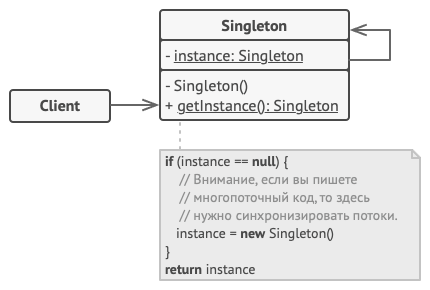
\includegraphics[scale=0.7]{images/pic/pic26-1.png}\caption{Cхема паттерна Singleton}\label{figure1}
\end{center}
\end{figure}
\newpage
\subsection{Пример использования}
\begin{lstlisting}
    class Singleton
    {
    private static Singleton uniqueInstance;
    privitae Singleton(){}
    public static Singleton getInstance()
        {
        if (uniqueInstance == null)
            uniqueInstance = new Singleton();
            return uniqueInstance;
        }
    }
\end{lstlisting}
В случае использования параллельных потоков, возможно создание нескольких экземпляров класса Singleton.
Решение: использование ключевого слова synchronized
\begin{lstlisting}
    class Singleton
    {
    private static Singleton uniqueInstance;
    privitae Singleton(){}
    public static synchronized Singleton getInstance()
        {
        if (uniqueInstance == null)
            uniqueInstance = new Singleton();
            return uniqueInstance;
        }
    }
\end{lstlisting}
Однако при использовании synchronized замедляется работа метода, что неприемлемо для интенсивно используемой части приложения.
Решение проблемы:
\begin{enumerate}
\item Оставить все как есть
\item Создать экземпляр заранее (если создание не сопряжено с затратами)
\item Воспользоваться «условной блокировкой»
\end{enumerate}
\begin{lstlisting}
    class Singleton
    {
    private static Singleton uniqueInstance = new Singleton();
    privitae Singleton(){}
    public static Singleton getInstance()
        {
            return uniqueInstance;
        }
    }
\end{lstlisting}

\section{Фабрика}
Паттерн Фабричный Метод определяет интерфейс создания объекта, но позволяет субклассам выбрать класс создаваемого экземпляра. Таким образом, Фабричный Метод делегирует операцию создания экземпляра субклассам.
\begin{figure}[!ht]
\begin{center}
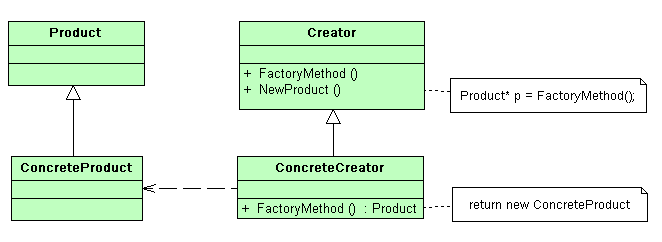
\includegraphics[scale=0.7]{images/pic/pic26-2.png}\caption{Cхема паттерна Фабрика}\label{figure1}
\end{center}
\end{figure}
\subsection{Пример использования}
\begin{lstlisting}
    abstract class Factory
        {
            public abstract Warrior createWarrior();
        };
    class InfantryFactory extends Factory
    {
        public Warrior createWarrior()
            {
                return new Infantryman();
            }
    };
    class ArchersFactory extends Factory
        {
            public Warrior createWarrior()
            {
                return new Archer();
            }
        };
    class CavalryFactory extends Factory
    {
        public Warrior createWarrior()
        {
        return new Horseman();
        }
    };
\end{lstlisting}
\section{Абстрактная фабрика}
Абстрактная фабрика — это порождающий паттерн проектирования, который позволяет создавать семейства связанных объектов, не привязываясь к конкретным классам создаваемых объектов.
\newpage
\begin{figure}[!ht]
\begin{center}
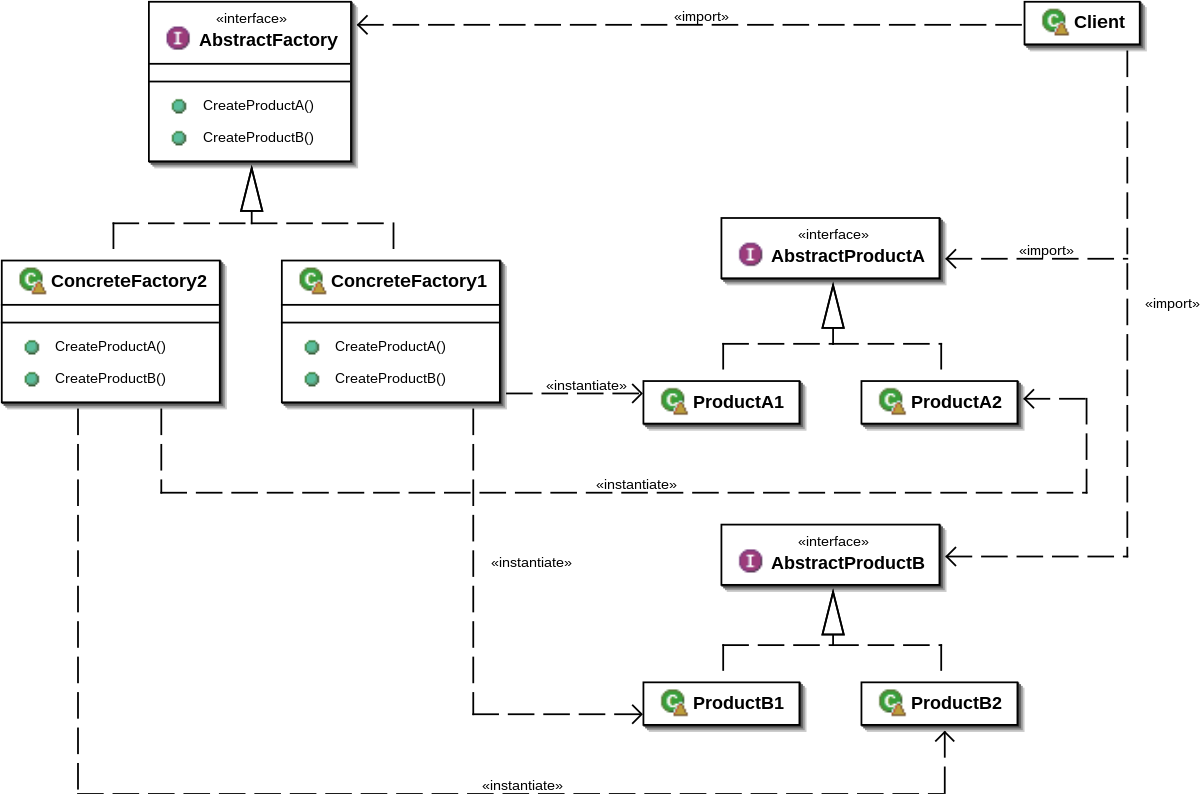
\includegraphics[scale=0.3]{images/pic/pic26-3.png}\caption{Cхема паттерна Абстрактная фабрика}\label{figure1}
\end{center}
\end{figure}

\subsection{Пример использования}
\begin{lstlisting}
   interface Button is
    method paint()

class WinButton implements Button is
    method paint() is

class MacButton implements Button is
    method paint() is

interface Checkbox is
    method paint()

class WinCheckbox implements Checkbox is
    method paint() is

class MacCheckbox implements Checkbox is
    method paint() is

interface GUIFactory is
    method createButton():Button
    method createCheckbox():Checkbox

class WinFactory implements GUIFactory is
    method createButton():Button is
        return new WinButton()
    method createCheckbox():Checkbox is
        return new WinCheckbox()

class MacFactory implements GUIFactory is
    method createButton():Button is
        return new MacButton()
    method createCheckbox():Checkbox is
        return new MacCheckbox()

class Application is
    private field factory: GUIFactory
    private field button: Button
    constructor Application(factory: GUIFactory) is
        this.factory = factory
    method createUI()
        this.button = factory.createButton()
    method paint()
        button.paint()

class ApplicationConfigurator is
    method main() is
        config = readApplicationConfigFile()

        if (config.OS == "Windows") then
            factory = new WinFactory()
        else if (config.OS == "Mac") then
            factory = new MacFactory()
        else
            throw new Exception("Error! Unknown operating system.")

        Application app = new Application(factory)
\end{lstlisting}

\newpage
\chapter{Структурные патттерны}
\section{Структурные паттерны и их основное свойство}
Структурные шаблоны (structural patterns) — шаблоны проектирования, в которых рассматривается вопрос о том, как из классов и объектов образуются более крупные структуры.

Проще говоря, структурные паттерны связаны с композицией объектов или тем, как сущности могут использовать друг друга.

\section{Создание сложных объектов из простых}
Структурные паттерны объединяют классы или объекты в более крупные структуры: они описывают способы объединения классов и объектов для создания новых структур и новой функциональности. Таким образом, их основной сутью является динамическое объединение объектов для расширения функциональности, а не взаимодействия между объектами, являющиеся содержанием поведенческих паттернов.

\section{Правила агрегации}
Объекты в пределах границы агрегации должны соответствовать следующим правилам:
    \begin{itemize}
    \item Непротиворечивость жизненного цикла
    \item Непротиворечивость проблемной области
    \item Постоянство частоты сценария
    \item Как можно меньше элементов в агрегации
    \end{itemize}

\section{Адаптер(Adapter)}
Паттерн Адаптер преобразует интерфейс класса к другому интерфейсу, на который рассчитан клиент. Адаптер обеспечивает совместную работу классов, невозможную в обычных условиях из-за несовместимости интерфейсов.
\begin{figure}[!ht]
\begin{center}
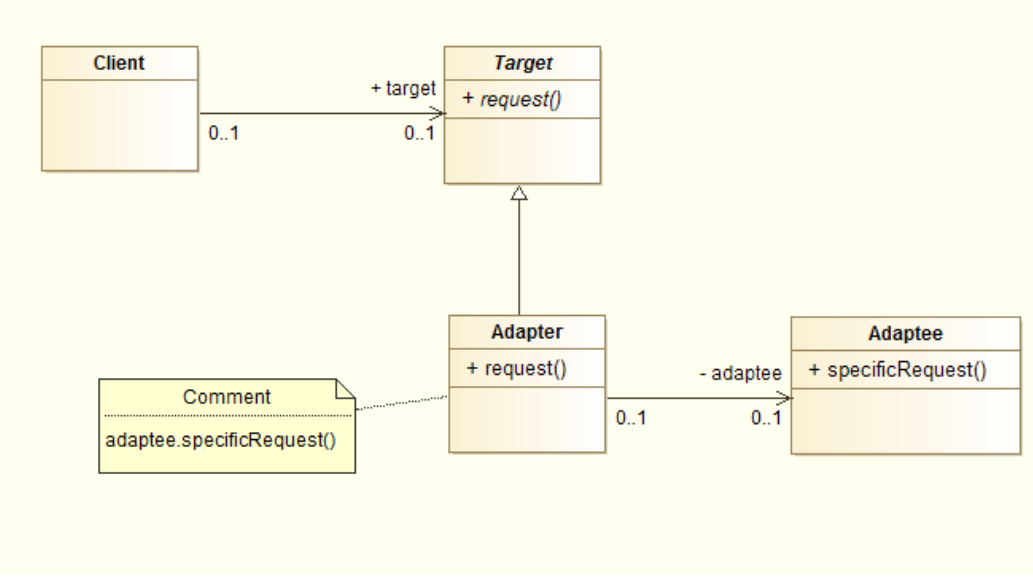
\includegraphics[scale=0.7]{images/pic/pic27-1.png}\caption{Cхема паттерна Адаптер}\label{figure1}
\end{center}
\end{figure}

\newpage
\subsection{Пример применения}
\begin{lstlisting}
    class FahrenheitSensor
    {
    public double getFahrenheitTemp()
    {
    double t = 32.0;
    //...
    return t;
    }
    
    interface Sensor
    {
        public double getTemperature();
    }
    class Adapter implements Sensor
    {
        FahrenheitSensor p fsensor;
        public Adapter(FahrenheitSensor p)
        {
            p_fsenser = p;
        }
        public double getTemperature()
        {
            return (p fsensor.getFahrenheitTemp()-32.0)*5.0/9.8;
        }
    }
    public class MainClass
    {
        public static void main(String[] args)
        {
            Sensor p = new Adapter(new FahrenheitSenser());
            System.out.println("Celsius temperature = " + p.getTemperature());
        }
    }
\end{lstlisting}

\section{Декоратор(Decorator)}

Паттерн Декоратор динамически наделяет объект новыми возможностями и является гибкой альтернативой субклассированию в области расширения функциональности
\begin{figure}[!ht]
\begin{center}
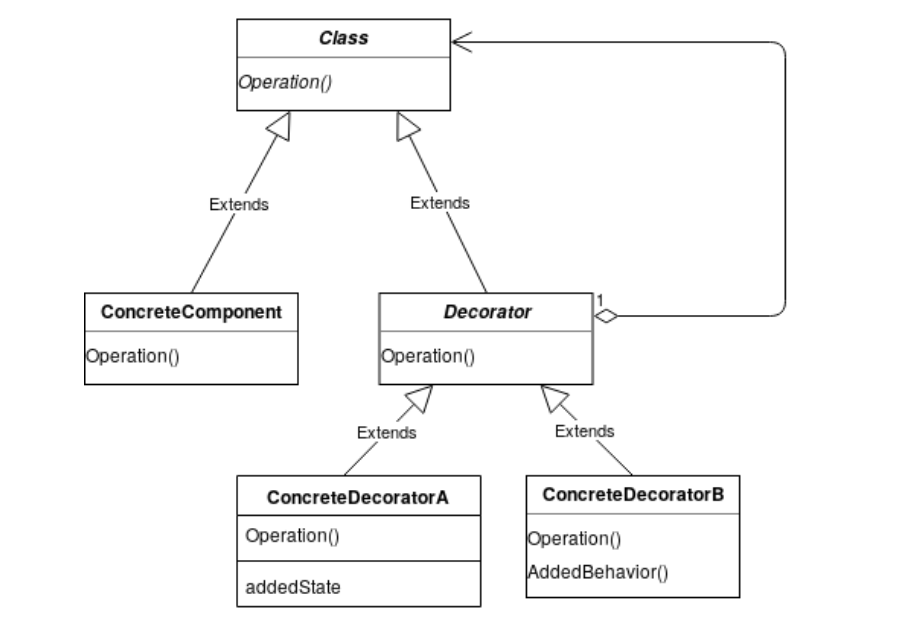
\includegraphics[scale=0.7]{images/pic/pic27-2.png}\caption{Cхема паттерна Декоратор}\label{figure1}
\end{center}
\end{figure}
\subsection{Роли классов в паттерне Декоратор}
 \begin{itemize}
    \item Component – компонент, определяет интерфейс для объектов, на которые могут быть возложены дополнительные обязанности.
    \item ConcreteComponent – конкретный компонент, определяет объект, на который могут быть возложены дополнительные обязанности.
    \item Decorator – декоратор, хранит ссылку на Component, определяет интерфейс, соответствующий интерфейсу Component.
    \item ConcreteDecorator – конкретный декоратор, возлагает дополнительные обязанности на компонент.
    \end{itemize}

\subsection{Результат применения паттерна Декоратор}
 \begin{itemize}
    \item Большая гибкость, чем при применении классического наследования. Можно добавлять и удалять обязанности во время выполнения программы. Декораторы можно сочетать произвольным образом, а также применять их многократно.
    \item Позволяет избежать перегруженных функциями классов на верхних уровнях иерархии. Уменьшает вероятность появления "Божественного объекта".
    \item Декоратор и его компонент не идентичны
    \item Множество мелких объектов.
    \end{itemize}
\subsection{Декоратор: особенности реализации}
\begin{itemize}
    \item соответствие интерфейсов - интерфейс Декоратора должен соответствовать интерфейсу декорируемого объекта
    \item отсутствие абстрактного класса Декоратор (если нужно добавить одну обязанность)
    \item облегченные классы Component. Важно, чтобы класс Component был настолько легким, насколько это возможно.
    \item изменение облика, а не внутреннего устройства объекта. Альтернатива – паттерн Стратегия (изменение внутреннего устройства объекта).
    \end{itemize}
\subsection{Пример применения}
\begin{lstlisting}
interface DataSource is
    method writeData(data)
    method readData():data
class FileDataSource implements DataSource is
    constructor FileDataSource(filename) { ... }

    method writeData(data) is

    method readData():data is

class DataSourceDecorator implements DataSource is
    protected field wrappee: DataSource

    constructor DataSourceDecorator(source: DataSource) is
        wrappee = source

    method writeData(data) is
        wrappee.writeData(data)

    method readData():data is
        return wrappee.readData()

class EncryptionDecorator extends DataSourceDecorator is
    method writeData(data) is

    method readData():data is

class CompressionDecorator extends DataSourceDecorator is
    method writeData(data) is

    method readData():data is

class Application is
    method dumbUsageExample() is
        source = new FileDataSource("somefile.dat")
        source.writeData(salaryRecords)

        source = new CompressionDecorator(source)
        source.writeData(salaryRecords)

        source = new EncryptionDecorator(source)

        source.writeData(salaryRecords)
\end{lstlisting}

\section{Компоновщик(Composite)}
Компонует объекты в древовидные структуры для представления иерархий
часть-целое. Позволяет клиентам единообразно трактовать индивидуальные
и составные объекты.
\begin{figure}[!ht]
\begin{center}
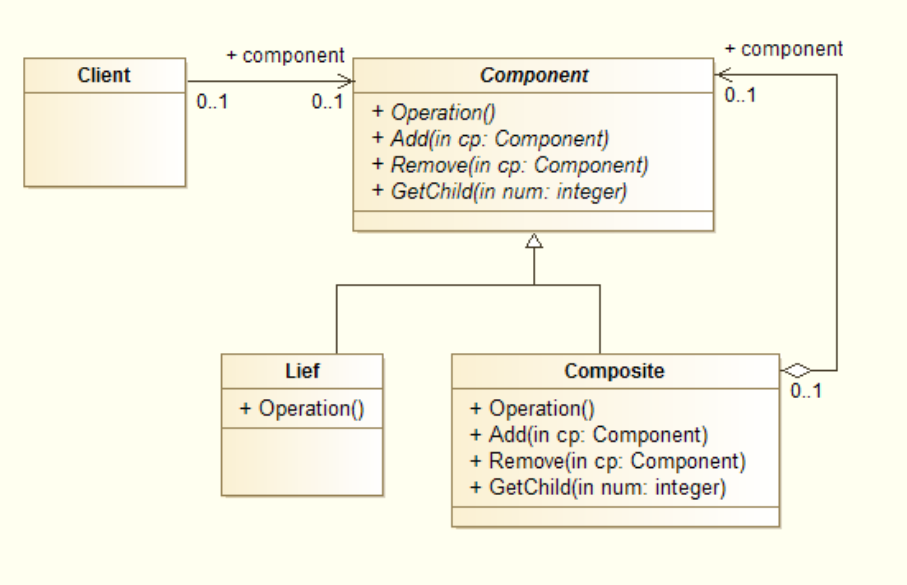
\includegraphics[scale=0.7]{images/pic/pic27-3.png}\caption{Cхема паттерна Компоновщик}\label{figure1}
\end{center}
\end{figure}
\subsection{Роли классов в паттерне Компоновщик}
\begin{itemize}
    \item Component – компонент: объявляет интерфейс для компонуемых объектов, предоставляет подходящую реализацию операций по умолчанию, объявляет интерфейс для доступа к потомках и управления ими, определяет интерфейс для доступа к родителю компонента в рекурсивной структуре и реализует его (необязательно)
    \item Leaf – лист: представляет листовые узлы композиции и не имеет потомков
    \item Composite – составной объект: определяет поведение компонентов, у которых есть потомки, хранит компоненты-потомки, реализует относящиеся к управлению потомками операции в интерфейсе класса Component
    \item Client – клиент: манипулирует объектами композиции через интерфейс Component
    \end{itemize}
\subsection{Компоновщик: особенности реализации}
\begin{itemize}
    \item Ссылки на родителей
    \item Разделение компонентов
    \item Максимизация интерфейса класса Component
    \item Объявление операций для управления потомками
    \item Список компонентов
    \item Упорядочивание потомков
    \item Кэширование
    \item Какую структуру использовать для хранения компонент
    \end{itemize}

\subsection{Пример использования}
\begin{lstlisting}
interface Graphic is
    method move(x, y)
    method draw()

class Dot implements Graphic is
    field x, y

    constructor Dot(x, y) { ... }

    method move(x, y) is
        this.x += x, this.y += y

    method draw() is

class Circle extends Dot is
    field radius

    constructor Circle(x, y, radius) { ... }

    method draw() is

class CompoundGraphic implements Graphic is
    field children: array of Graphic

    method add(child: Graphic) is

    method remove(child: Graphic) is

    method move(x, y) is
        foreach (child in children) do
            child.move(x, y)

    method draw() is

class ImageEditor is
    field all: CompoundGraphic

    method load() is
        all = new CompoundGraphic()
        all.add(new Dot(1, 2))
        all.add(new Circle(5, 3, 10))
        // ...

    method groupSelected(components: array of Graphic) is
        group = new CompoundGraphic()
        foreach (component in components) do
            group.add(component)
            all.remove(component)
        all.add(group)
        all.draw()
\end{lstlisting}

\section{Мост(Bridge)}
Мост – это структурный паттерн проектирования, который разделяет один
или несколько классов на две отдельные иерархии – абстракцию и
реализацию, позволяя изменять их независимо друг от друга.
Мост – паттерн, структурирующий объекты.
\begin{figure}[!ht]
\begin{center}
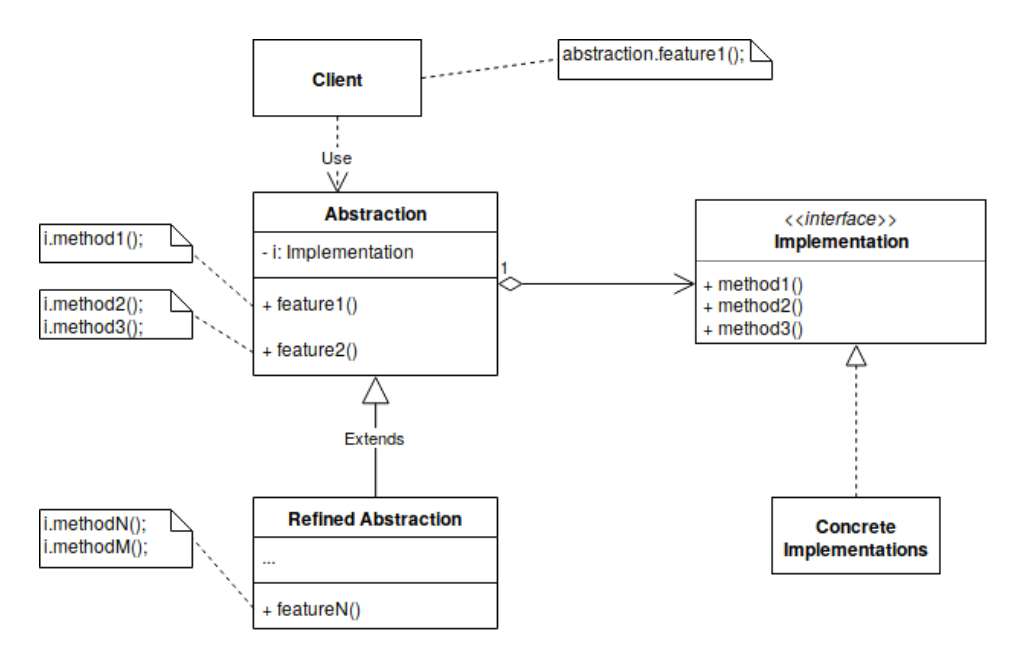
\includegraphics[scale=0.7]{images/pic/pic27-4.png}\caption{Cхема паттерна Мост}\label{figure1}
\end{center}
\end{figure}

\subsection{Роли классов в паттерне Мост}
\begin{itemize}
    \item Abstraction – абстракция, определяет интерфейс абстракции, хранит ссылку на объект типа Implementation
    \item Refined Abstraction – уточненная абстракция, расширяет интерфейс Abstraction.
    \item Implementation – реализатор, определяет интерфейс для классов реализации. Обычно интерфейс класса Implementation предоставляет только примитивные операции, а класс Abstraction определяет операции более высокого уровня, базирующийся на этих примитивах.
    \item Concrete Implementations – конкретные реализаторы. Содержат конкретные реализации интерфейса класса Implementation.
    \item Client – манипулирует объектами реализации через интерфейс абстракции.
\end{itemize}
\subsection{Пример применения}
\begin{lstlisting}
    class Remote is
    protected field device: Device
    constructor Remote(device: Device) is
        this.device = device
    method togglePower() is
        if (device.isEnabled()) then
            device.disable()
        else
            device.enable()
    method volumeDown() is
        device.setVolume(device.getVolume() - 10)
    method volumeUp() is
        device.setVolume(device.getVolume() + 10)
    method channelDown() is
        device.setChannel(device.getChannel() - 1)
    method channelUp() is
        device.setChannel(device.getChannel() + 1)

class AdvancedRemote extends Remote is
    method mute() is
        device.setVolume(0)

interface Device is
    method isEnabled()
    method enable()
    method disable()
    method getVolume()
    method setVolume(percent)
    method getChannel()
    method setChannel(channel)

class Tv implements Device is
    // ...

class Radio implements Device is
    // ...

tv = new Tv()
remote = new Remote(tv)
remote.togglePower()

radio = new Radio()
remote = new AdvancedRemote(radio)
\end{lstlisting}


\newpage
\chapter{Поведенчиские паттерны}

\subsection{Поведенческие паттерны и их основное свойство}
Поведенческие паттерны проектирования предназначены для решения задач организации эффективного и безопасного взаимодействия между объектами разрабатываемой системы. Они больше остальных паттернов связаны с алгоритмами и способами распределения обязанностей между объектами.

\section{Абстракция поведения}
Абстракция выделяет существенные характеристики некоторого объекта, отличающие его от всех других видов объектов и, таким образом, четко определяет его концептуальные границы с точки зрения наблюдателя.
Абстрагирование концентрирует внимание на внешних особенностях объекта и позволяет отделить самые существенные особенности поведения от несущественных. Такое разделение основывается на принципе минимизации связей, когда интерфейс объекта содержит только существенные аспекты поведения и ничего больше. Выбор правильного набора абстракций для заданной предметной области представляет собой главную задачу ОО проектирования. 

\section{Стратегия}
Определяет семейство алгоритмов, инкапсулирует каждый из них и делает их
взаимозаменяемыми. Стратегия позволяет изменять алгоритмы независимо
от клиентов, которые ими пользуются.
\begin{figure}[!ht]
\begin{center}
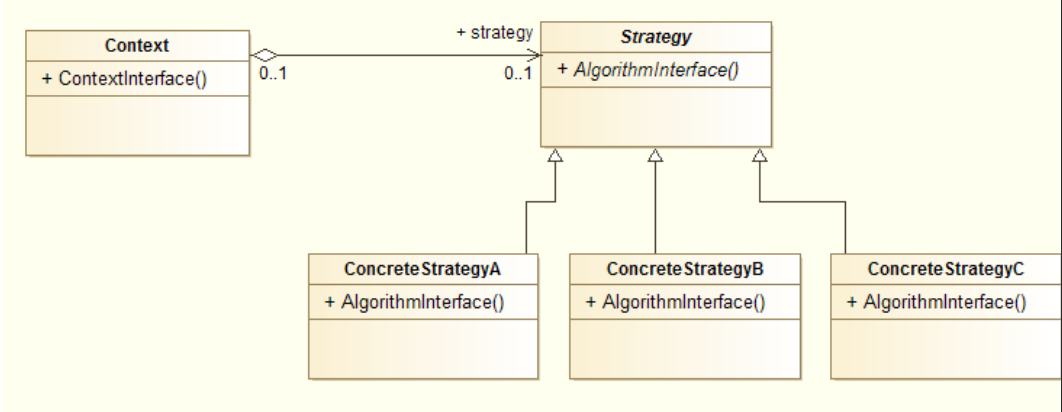
\includegraphics[scale=0.7]{images/pic/pic28-1.png}\caption{Cхема паттерна Стратегия}\label{figure1}
\end{center}
\end{figure}
\subsection{Strategy: роли классов}
\begin{itemize}
    \item Strategy – стратегия: объявляет общий для всех поддерживаемых алгоритмов интерфейс. Класс Context пользуется этим интерфейсом для вызова конкретного алгоритма, определенного в классе
    \item ConcreteStrategy – конкретная стратегия: реализует алгоритм, использующий интерфейс, объявленный в классе Strategy.
    \item Context – контекст: конфигурируется объектом класса
    \item ConcreteStrategy, хранит ссылку на объект класса Strategy, может определять интерфейс, который позволяет объекту Strategy получить доступ к данным контекста.
\end{itemize}
\subsection{Strategy: результаты применения}
\begin{itemize}
    \item Семейства родственных алгоритмов
    \item Альтернатива порождению подклассов
    \item С помощью стратегий можно избавиться от условных операторов
    \item Выбор реализации
    \item Клиенты должны ¾знать¿ о различных стратегиях
    \item Обмен информацией между стратегией и контекстом
    \item Увеличение числа объектов
\end{itemize}
\subsection{Strategy: особенности реализации}
\begin{itemize}
    \item Определение интерфейсов классов Strategy и Context
    \item Стратегии как обобщенный тип для контекста
    \item Объекты-стратегии можно не задавать
\end{itemize}
\begin{lstlisting}
    interface Strategy is
    method execute(a, b)

class ConcreteStrategyAdd implements Strategy is
    method execute(a, b) is
        return a + b

class ConcreteStrategySubtract implements Strategy is
    method execute(a, b) is
        return a - b

class ConcreteStrategyMultiply implements Strategy is
    method execute(a, b) is
        return a * b

class Context is
    private strategy: Strategy

    method setStrategy(Strategy strategy) is
        this.strategy = strategy

    method executeStrategy(int a, int b) is
        return strategy.execute(a, b)

class ExampleApplication is
    method main() is

        if (action == addition) then
            context.setStrategy(new ConcreteStrategyAdd())

        if (action == subtraction) then
            context.setStrategy(new ConcreteStrategySubtract())

        if (action == multiplication) then
            context.setStrategy(new ConcreteStrategyMultiply())

        result = context.executeStrategy(n1, n2)
\end{lstlisting}

\section{Итератор}
Предоставляет способ последовательного доступа ко всем элементам
составного объекта, не раскрывая его внутреннего представления
\begin{figure}[!ht]
\begin{center}
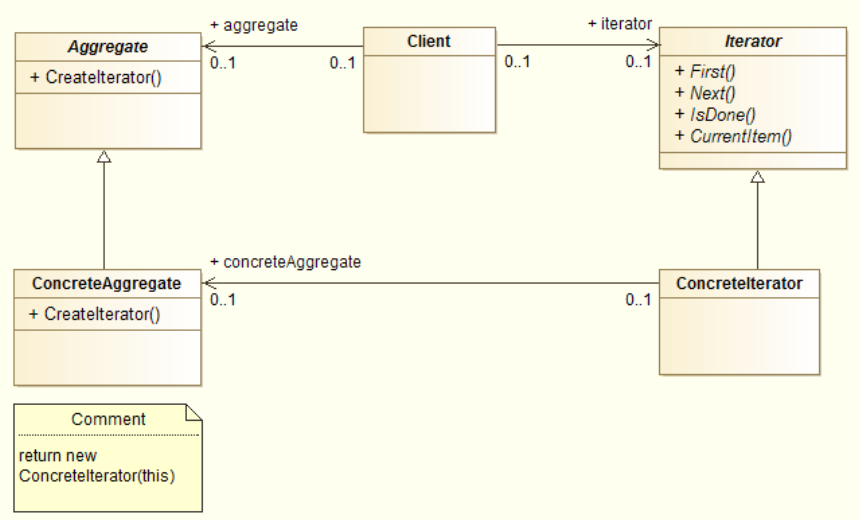
\includegraphics[scale=0.7]{images/pic/pic28-2.png}\caption{Cхема паттерна Итератор}\label{figure1}
\end{center}
\end{figure}
\subsection{Роли классов}
\begin{itemize}
    \item Iterator – итератор: определяет интерфейс для доступа и обхода элементов
    \item ConcreteIterator – конкретный итератор: реализует интерфейс класса
    \item Iterator, следит за текущей позицией при обходе агрегата
    \item Aggregate – агрегат: определяет интерфейс для создания объекта-итератора
    \item ConcreteAggregate – конкретный агрегат: реализует интерфейс создания итератора и возвращает экземпляр подходящего класса
\end{itemize}
\subsection{Результат применения}
\begin{itemize}
    \item Поддержка различных видов обхода агрегата
    \item Итераторы упрощают интерфейс класса Aggregate
    \item Одновременно для данного агрегата может быть активно несколько обходов
\end{itemize}
\subsection{Итератор: особенности реализации}
\begin{itemize}
    \item Какой участник управляет итерацией?
    \item Что определяет алгоритм обхода?
    \item Насколько итератор устойчив?
    \item Дополнительные операции итератора
    \item Итераторы для составных объектов
    \item Пустые итераторы
\end{itemize}
\subsection{Итератор: пример применения}
\begin{lstlisting}
class Facebook implements SocialNetwork is

    method createFriendsIterator(profileId) is
        return new FacebookIterator(this, profileId, "friends")
    method createCoworkersIterator(profileId) is
        return new FacebookIterator(this, profileId, "coworkers")

interface ProfileIterator is
    method getNext():Profile
    method hasMore():bool

class FacebookIterator implements ProfileIterator is
    private field facebook: Facebook
    private field profileId, type: string

    private field currentPosition
    private field cache: array of Profile

    constructor FacebookIterator(facebook, profileId, type) is
        this.facebook = facebook
        this.profileId = profileId
        this.type = type

    private method lazyInit() is
        if (cache == null)
            cache = facebook.socialGraphRequest(profileId, type)

    method getNext() is
        if (hasMore())
            currentPosition++
            return cache[currentPosition]

    method hasMore() is
        lazyInit()
        return currentPosition < cache.length

class SocialSpammer is
    method send(iterator: ProfileIterator, message: string) is
        while (iterator.hasMore())
            profile = iterator.getNext()
            System.sendEmail(profile.getEmail(), message)

class Application is
    field network: SocialNetwork
    field spammer: SocialSpammer

    method config() is
        if working with Facebook
            this.network = new Facebook()
        if working with LinkedIn
            this.network = new LinkedIn()
        this.spammer = new SocialSpammer()

    method sendSpamToFriends(profile) is
        iterator = network.createFriendsIterator(profile.getId())
        spammer.send(iterator, "Very important message")

    method sendSpamToCoworkers(profile) is
        iterator = network.createCoworkersIterator(profile.getId())
        spammer.send(iterator, "Very important message")
\end{lstlisting}

\section{Состояние (State)}
Позволяет объекту варьировать свое поведение в зависимости от внутреннего
состояния. Извне создается впечатление, что изменился класс объекта.
\begin{figure}[!ht]
\begin{center}
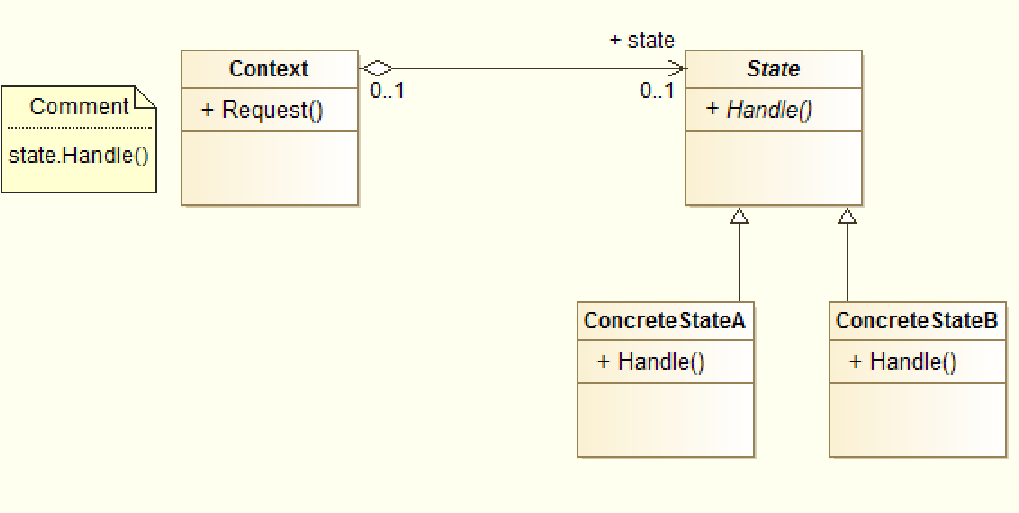
\includegraphics[scale=0.7]{images/pic/pic28-3.png}\caption{Cхема паттерна Состояние}\label{figure1}
\end{center}
\end{figure}
\subsection{Состояние: роли классов}
\begin{itemize}
    \item Context – контекст: определяет интерфейс, представляющий интерес для клиентов, хранит экземпляр подкласса ConcreteState, которым определяется текущее состояние
     \item State – состояние: определяет интерфейс для инкапсуляции поведения, ассоциированного с конкретным состоянием контекста Context
     \item Подклассы ConcreteState – конкретное состояние: каждый подкласс реализует поведение, ассоциированное с некоторым состоянием контекста Context.
\end{itemize}
\subsection{Состояние: результат применения}
\begin{itemize}
    \item Локализует зависящее от состояния поведение и делит его на части, соответствующие состояниям
    \item Делает явными переходы между состояниями
    \item Объекты состояния можно разделять
\end{itemize}
\subsection{Состояние: особенности реализации}
\begin{itemize}
    \item Что определяет переходы между состояниями
    \item Табличная альтернатива
    \item Создание объектов состояния
\end{itemize}
\subsection{Состояние: пример применения}
\begin{lstlisting}
abstract class State is
    protected field player: AudioPlayer

    constructor State(player) is
        this.player = player

    abstract method clickLock()
    abstract method clickPlay()
    abstract method clickNext()
    abstract method clickPrevious()

class LockedState extends State is

    method clickLock() is
        if (player.playing)
            player.changeState(new PlayingState(player))
        else
            player.changeState(new ReadyState(player))

    method clickPlay() is

    method clickNext() is

    method clickPrevious() is

class ReadyState extends State is
    method clickLock() is
        player.changeState(new LockedState(player))

    method clickPlay() is
        player.startPlayback()
        player.changeState(new PlayingState(player))

    method clickNext() is
        player.nextSong()

    method clickPrevious() is
        player.previousSong()


class PlayingState extends State is
    method clickLock() is
        player.changeState(new LockedState(player))

    method clickPlay() is
        player.stopPlayback()
        player.changeState(new ReadyState(player))

    method clickNext() is
        if (event.doubleclick)
            player.nextSong()
        else
            player.fastForward(5)

    method clickPrevious() is
        if (event.doubleclick)
            player.previous()
        else
            player.rewind(5)

class AudioPlayer is
    field state: State
    field UI, volume, playlist, currentSong

    constructor AudioPlayer() is
        this.state = new ReadyState(this)

        UI = new UserInterface()
        UI.lockButton.onClick(this.clickLock)
        UI.playButton.onClick(this.clickPlay)
        UI.nextButton.onClick(this.clickNext)
        UI.prevButton.onClick(this.clickPrevious)

    method changeState(state: State) is
        this.state = state

    method clickLock() is
        state.clickLock()
    method clickPlay() is
        state.clickPlay()
    method clickNext() is
        state.clickNext()
    method clickPrevious() is
        state.clickPrevious()

    method startPlayback() is
        // ...
    method stopPlayback() is
        // ...
    method nextSong() is
        // ...
    method previousSong() is
        // ...
    method fastForward(time) is
        // ...
    method rewind(time) is
        // ...
\end{lstlisting}

\section{Команда (Command)}
Инкапсулирует запрос как объект, позволяя тем самым задавать параметры
клиентов для обработки соответствующих запросов, ставить запросы в
очередь или протоколировать их, а также поддерживать отмену операций.
\begin{figure}[!ht]
\begin{center}
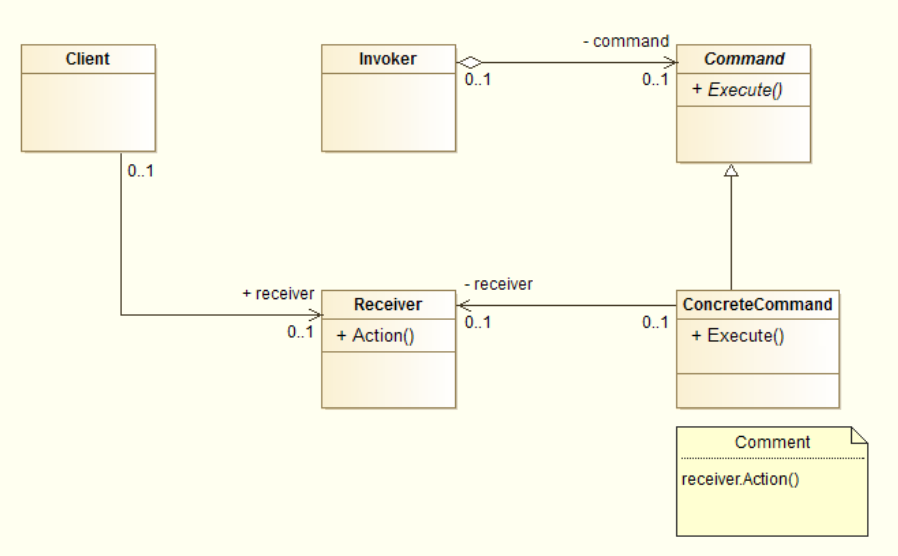
\includegraphics[scale=0.7]{images/pic/pic28-4.png}\caption{Cхема паттерна Состояние}\label{figure1}
\end{center}
\end{figure}
\subsection{Команда: роли классов}
\begin{itemize}
    \item Command – команда: объявляет интерфейс для выполнения операции
    \item ConcreteCommand – конкретная команда: определяет связь между объектом-получателем Receiver и действием, реализует операцию
    \item Execute путем вызова соответствующих операций объекта Receiver
    \item Client – клиент : создает объект класса ConcreteCommand и устанавливает его получателя
    \item Invoker – инициатор: обращается к команде для выполнения запроса
    \item Receiver – получатель: располагает информацией о способах выполнения операций, необходимых для удовлетворения запроса. В роли получателя может выступать любой класс.
\end{itemize}
\subsection{Команда: результат применения}
\begin{itemize}
    \item Команда разрывает связь между объектом, инициирующем операцию, и объектом, имеющим информацию о том, как ее выполнить
    \item Команды – это объекты. Допускаются любые манипуляции, присущие объектам.
    \item Можно создать MacroCommand. Такие команды описываются Composite.
    \item Легко добавить новые команды.
\end{itemize}
\subsection{Команда: особенности реализации}
\begin{itemize}
    \item Насколько умной должна быть команда?
    \item Поддержка отмены и повтора операций
    \item Как избежать ошибок в процессе отмены?
    \item Применение обобщенных типов для команд, не допускающих отмену и не имеющих аргументов
\end{itemize}
\subsection{Команда: пример применения}
\begin{lstlisting}
abstract class Command is
    protected field app: Application
    protected field editor: Editor
    protected field backup: text

    constructor Command(app: Application, editor: Editor) is
        this.app = app
        this.editor = editor

    method saveBackup() is
        backup = editor.text

    method undo() is
        editor.text = backup

    abstract method execute()

class CopyCommand extends Command is

    method execute() is
        app.clipboard = editor.getSelection()
        return false

class CutCommand extends Command is

    method execute() is
        saveBackup()
        app.clipboard = editor.getSelection()
        editor.deleteSelection()
        return true

class PasteCommand extends Command is
    method execute() is
        saveBackup()
        editor.replaceSelection(app.clipboard)
        return true

class UndoCommand extends Command is
    method execute() is
        app.undo()
        return false

class CommandHistory is
    private field history: array of Command

    method push(c: Command) is

    method pop():Command is

class Editor is
    field text: string

    method getSelection() is

    method deleteSelection() is

    method replaceSelection(text) is

class Application is
    field clipboard: string
    field editors: array of Editors
    field activeEditor: Editor
    field history: CommandHistory

    method createUI() is
        // ...
        copy = function() {executeCommand(
            new CopyCommand(this, activeEditor)) }
        copyButton.setCommand(copy)
        shortcuts.onKeyPress("Ctrl+C", copy)

        cut = function() { executeCommand(
            new CutCommand(this, activeEditor)) }
        cutButton.setCommand(cut)
        shortcuts.onKeyPress("Ctrl+X", cut)

        paste = function() { executeCommand(
            new PasteCommand(this, activeEditor)) }
        pasteButton.setCommand(paste)
        shortcuts.onKeyPress("Ctrl+V", paste)

        undo = function() { executeCommand(
            new UndoCommand(this, activeEditor)) }
        undoButton.setCommand(undo)
        shortcuts.onKeyPress("Ctrl+Z", undo)

    method executeCommand(command) is
        if (command.execute())
            history.push(command)

    method undo() is
        command = history.pop()
        if (command != null)
            command.undo()
\end{lstlisting}
%--------------------------------------------------------------------------------------------

\section*{Вопросы и задания для самоконтроля}% Этот раздел будет состоять из вопросов
% и заданий для самоконтроля.
\addcontentsline{toc}{struct}{Вопросы и задания для самоконтроля}% Эта команда
% добавляет название раздела в раздел <<Содержание>>

Здесь можете привести список вопросов и заданий для самоконтроля:
\begin{enumerate}% Эта команда начинает список
\item Вопрос или задание.
\item Вопрос или задание.
\item Вопрос или задание.
\item Вопрос или задание.
\end{enumerate}% Эта команда завершает список

А можете подготовить с помощью программы IrenEditor (см. <<Руководство пользователю>>)
тестовое задание для самоконтроля, сохранить его в папку
<<test>>, назвав, например, lk1.exe, и создать на него метку с помощью
команды (см. <<Руководство пользователю>>): \href{run:test/lk1.exe}{Пройдем тестирование?}
